
\subsection{Vuelo y dispersión}
\label{subsec:cap4-vuelo-dispersion}
El Aedes aegypti es un mosquito doméstico que generalmente esta confinado a las casas donde se
cría \cite{luevano1993ciclo}, tiende a permanecer físicamente en donde emergió, siempre y cuando
no exista algún factor que la perturbe o no disponga de huéspedes, sitios de reposo y de postura
\cite{ThironIzcazaJ2003}. Por lo general, el mosquito, no sobrepasa los 50 a 100 metros durante su
vida \cite{cabezas2005dengue}. En caso de no contar con sitios adecuados de ovipostura y
disponibilidad de alimento tienden a dispersarme una mayor distancia, hasta tres kilómetros, en
busca de mejores condiciones \cite{ThironIzcazaJ2003}. Los mosquitos tienen la particularidad de
volar en sentido contrario a la dirección al viento \cite{ThironIzcazaJ2003,web-site:speedAnimals}
y a una velocidad máxima de 2 kilómetros por hora \cite{web-site:speedAnimals,kaufmann2004flight}.

Existen varios factores externos, que influyen el la dispersión del mosquito, disponibilidad de
alimentos, criaderos, sitios de reposo. Para las estrategias de control del Aedes aegypti en zonas
urbanas donde existen brotes de dengue y fiebre amarilla se asume que los mosquitos tienen un
rango de vuelo durante su vida de 50 a 100 metros \cite{dengueUruguayCap8}.

La función más importante del adulto del Aedes aegypti es la reproducción y secundariamente la
dispersión de la especie \cite{ThironIzcazaJ2003}. Para el Aedes aegypti el transporte pasivo de
huevos y larvas en recipientes ha tenido mayor trascendencia en su distribución, en la que el
hombre ha participado en forma determinante en comparación con la dispersión activa propia de la
especie \citep{ThironIzcazaJ2003}.

Partiendo de las hipótesis realizadas en la \secref{subsec:cap4-zonificacion} podemos considerar
que la dispersión se encuentra influenciada por el valor de $u(x,y)$, de ese modo a medida que
$u(x,y)$ varíe, la dispersión debe ajustarse a su tipo de zona. De forma simplificada definimos que
la dispersión de un adulto que se encuentre en zonas del tipo \textit{Regular}, \textit{Buena} u
\textit{Óptima} se encuentra entre 0 y 100 metros de vuelo. Para las hembras adultas, que
pertenezcan a zonas del tipo \textit{Mala} o \textit{Pésima} se tiene una dispersión entre 100 a
3.000 metros de vuelo, de este modo, las hembras adultas que se encuentren en zonas menos aptas
tenderán a desplazarse en busca de mejores condiciones (\figref{fig:cap4-dispersion}).

\begin{figure}[!hptb]
\centering
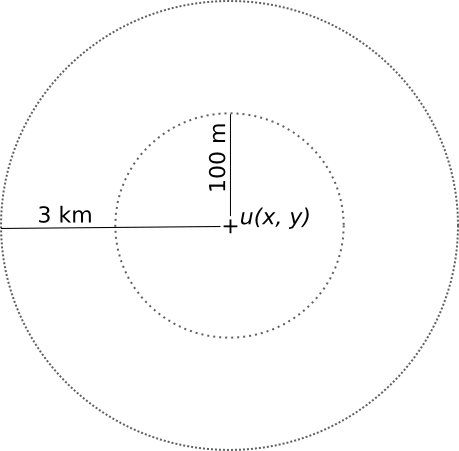
\includegraphics[width=0.4\textwidth]{capitulo-4/graphics/rango-vuelo.png}
\caption{\label{fig:cap4-dispersion} Rangos de dispersión del vector.}
\end{figure}
